\section{Contextualiser}

\begin{frame}{Le bloc opératoire, une ressource rare et non stockable}
  \small
  \begin{columns}[T,onlytextwidth]
    \begin{column}{0.41\textwidth}
      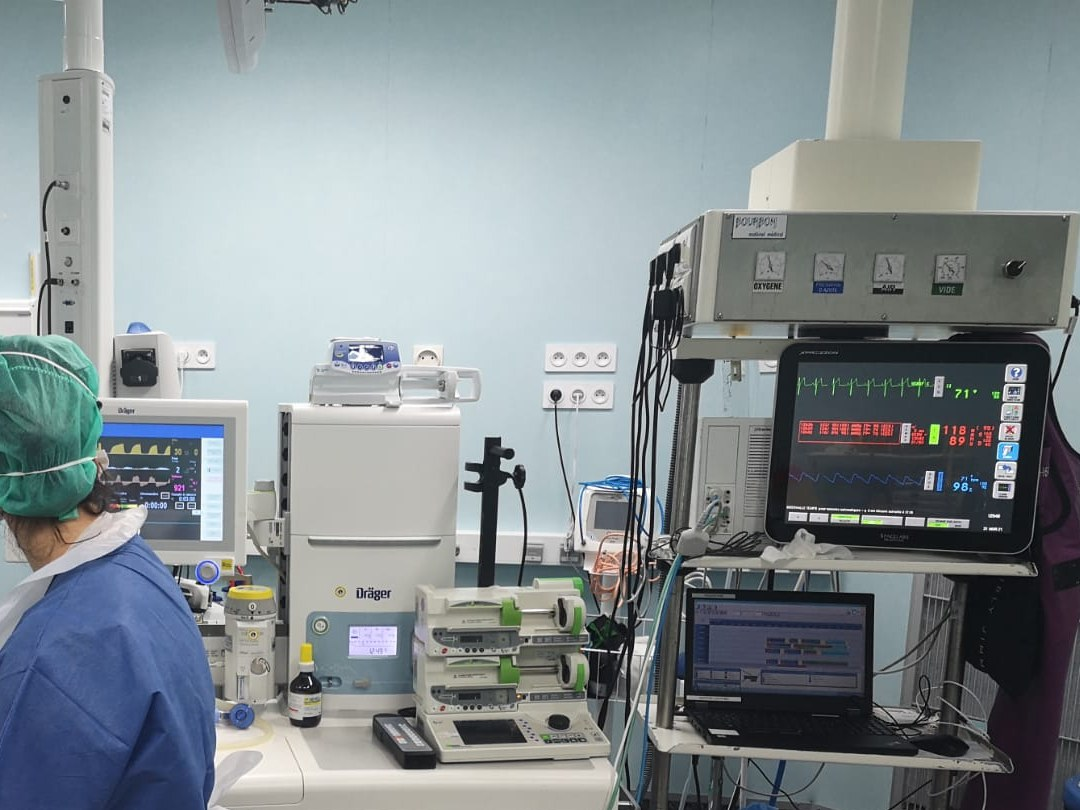
\includegraphics[width=\linewidth]{photo_bloc.jpg}
      \credit{Photo : Hirondus, CC BY-SA 4.0, Wikimedia Commons.}
    \end{column}

    \begin{column}{0.55\textwidth}
      \begin{columns}[T,onlytextwidth]
        \begin{column}{0.32\textwidth}\centering
          \bigstat{64,4\,\%}{taux national d'ambulatoire en 2023}
        \end{column}
        \begin{column}{0.32\textwidth}\centering
          \bigstat{70\,\%}{objectif national fixé pour 2022}
        \end{column}
        \begin{column}{0.32\textwidth}\centering
          \bigstat{80\,\%}{cap affiché pour la suite}
        \end{column}
      \end{columns}

      \uncover<2->{%
      \vspace{0.18cm}
      \begin{block}{Enjeux}
        \footnotesize
        Une salle, une équipe et un lit mobilisés sans patient coûtent sans
        soigner. L'objectif national et l'autorisation ARS rendent la décision
        traçable ; l'ambulatoire réduit le risque infectieux et accélère
        l'accès.
      \end{block}}
    \end{column}
  \end{columns}
  \source{Sources : HAS, IQSS (avril 2026) ; HAS, 12 questions (2012).}
\end{frame}

\begin{frame}{Du flux poussé au flux tiré}
  \scriptsize
  \begin{columns}[T,onlytextwidth]
    \begin{column}{0.58\textwidth}
      \only<1>{%
      \begin{block}{Aujourd'hui : flux poussé}
        \centering
        \begin{tikzpicture}[
          b/.style={draw=McmTerracotta,rounded corners=2pt,fill=white,
                    text width=1.85cm,minimum height=1.0cm,align=center,
                    font=\scriptsize,inner sep=2pt},
          f/.style={-{Latex[length=2mm]},thick,draw=McmTerracotta}]
          \node[b] (a) at (0,0) {Le chirurgien\\choisit une date};
          \node[b] (b) at (3.0,0) {Bloc, lits et\\équipes s'adaptent};
          \node[b] (c) at (6.0,0) {Pics et creux\\d'activité};
          \draw[f] (a) -- (b);
          \draw[f] (b) -- (c);
        \end{tikzpicture}
      \end{block}}

      \only<2->{%
      \begin{exampleblock}{Demain : flux tiré}
        \centering
        \begin{tikzpicture}[
          b/.style={draw=McmSage,rounded corners=2pt,fill=white,
                    text width=1.85cm,minimum height=1.0cm,align=center,
                    font=\scriptsize,inner sep=2pt},
          f/.style={-{Latex[length=2mm]},thick,draw=McmSage}]
          \node[b] (a) at (0,0) {Ressources et\\contraintes};
          \node[b] (b) at (3.0,0) {Dates A et B\\calculées};
          \node[b] (c) at (6.0,0) {Le chirurgien\\choisit};
          \draw[f] (a) -- (b);
          \draw[f] (b) -- (c);
        \end{tikzpicture}
      \end{exampleblock}}

      \uncover<3->{\par\vspace{0.15cm}\centering\footnotesize
        Le planning propose des dates compatibles ; le praticien arbitre.}
    \end{column}

    \begin{column}{0.40\textwidth}
      \centering
      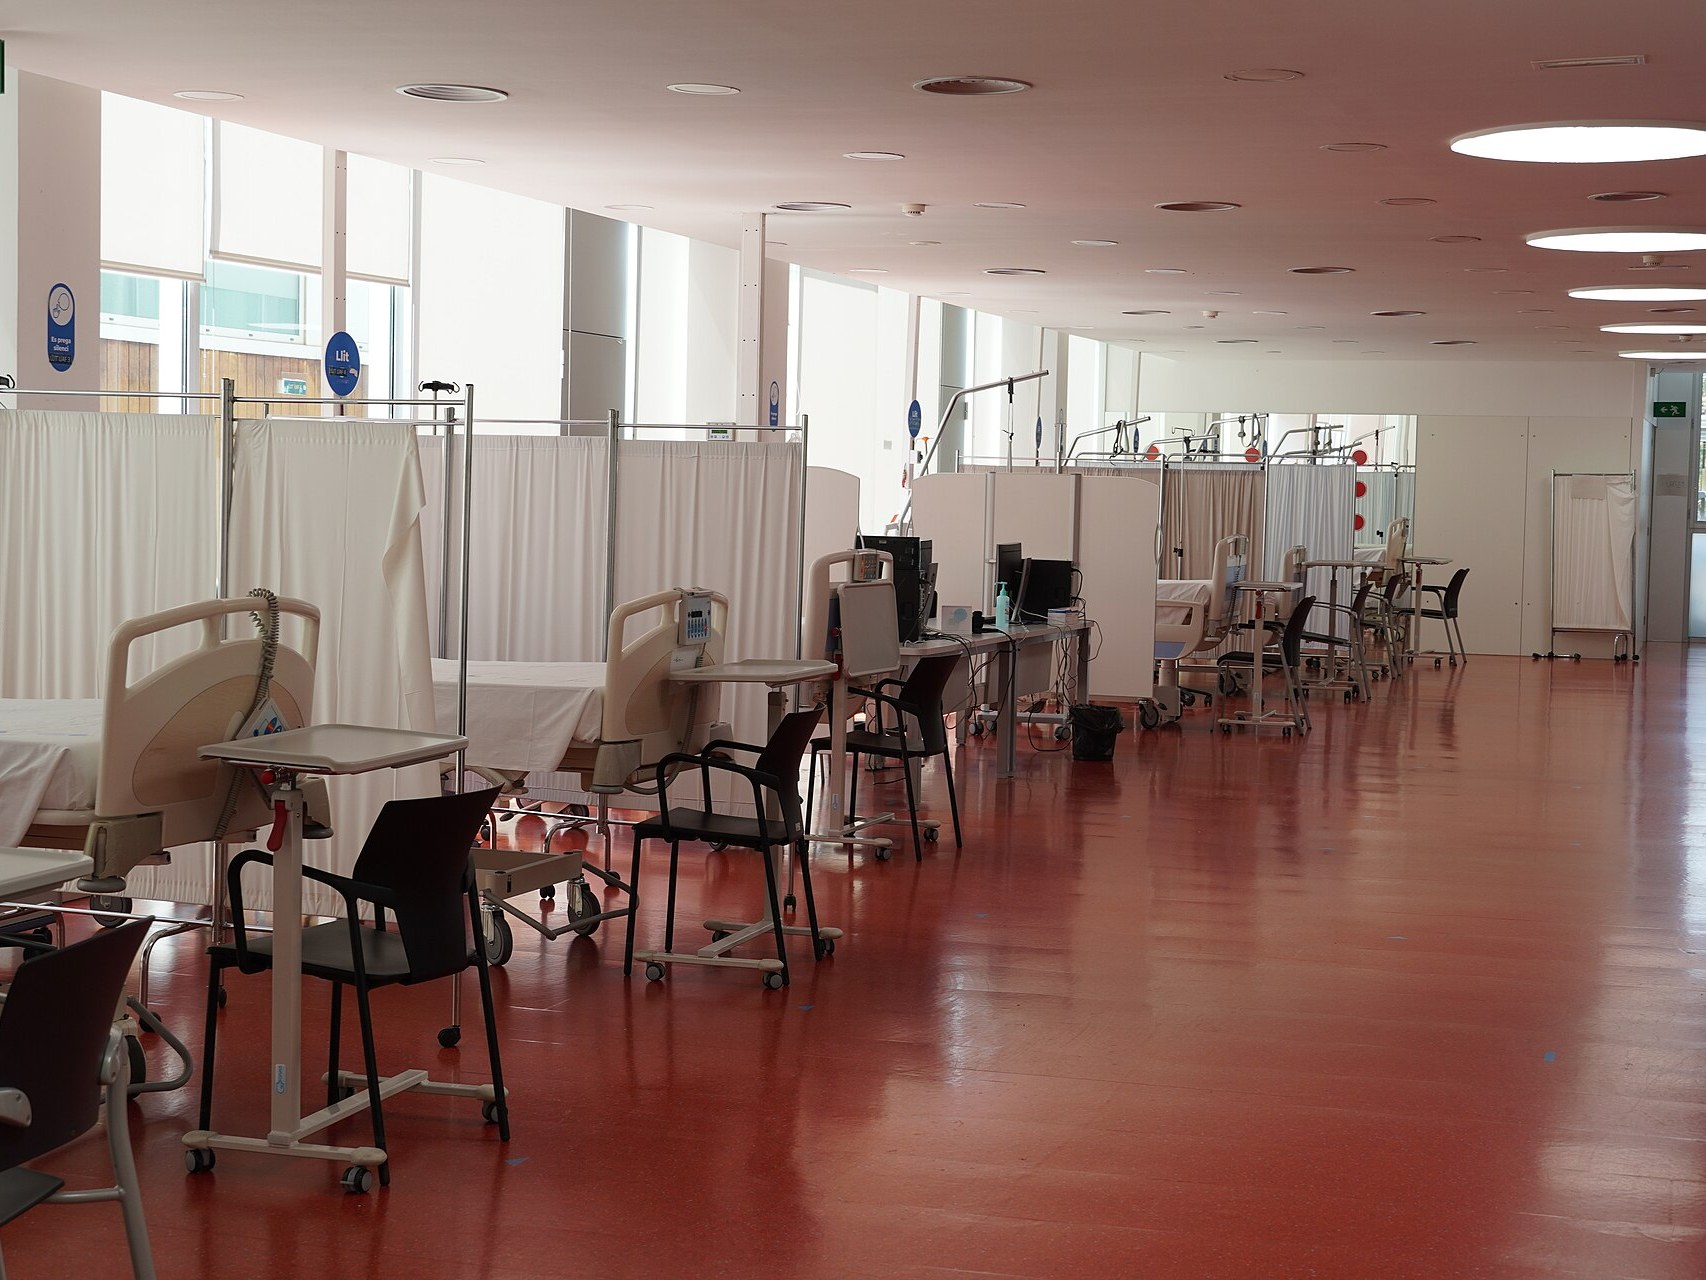
\includegraphics[width=0.88\linewidth]{photo_lits.jpg}
      \credit{Photo : Ncsi24, CC BY-SA 4.0, Wikimedia Commons.}
      \par\vspace{0.12cm}
      {\footnotesize Un séjour de plusieurs jours engage la capacité de
        demain.}
    \end{column}
  \end{columns}
\end{frame}

\begin{frame}{Ce que fait l'application, et ce qu'elle ne fait pas}
  \small
  \begin{columns}[T,onlytextwidth]
    \begin{column}{0.56\textwidth}
      \begin{enumerate}
        \item<1-> Le chirurgien saisit la demande en consultation.
        \item<1-> Le moteur prédit les durées et l'hébergement.
        \item<2-> L'outil propose \textbf{deux dates}, avec leurs raisons.
        \item<2-> Le chirurgien confirme : vacation et lit sont réservés.
      \end{enumerate}

      \uncover<3->{\par\vspace{0.15cm}\footnotesize
        L'outil ne programme pas à la place du praticien. Il rend les
        conséquences d'un choix visibles avant la confirmation.}
    \end{column}

    \begin{column}{0.42\textwidth}
      \centering
      \begin{tikzpicture}[font=\scriptsize]
        \draw[rounded corners=9pt,fill=white,draw=McmTerracotta,thick]
          (0,0) rectangle (4.15,6.05);
        \draw[fill=McmTerracotta!10,rounded corners=4pt]
          (0.18,5.35) rectangle (3.97,5.90);
        \node[font=\footnotesize\bfseries,text=McmTerracotta] at (2.08,5.62)
          {Demande};
        \node[align=left,anchor=west] at (0.28,4.95)
          {\textbf{Mme D., 58 ans}\\Chirurgie digestive};
        \draw[draw=McmMuted!35] (0.25,4.55) -- (3.90,4.55);
        \node[align=left,anchor=west] at (0.28,4.25)
          {Durée prédite : \textbf{95 min}\\Séjour : \textbf{2 jours}};
        \draw[fill=McmSage!12,rounded corners=3pt]
          (0.25,2.75) rectangle (3.90,3.95);
        \node[align=left,anchor=west] at (0.35,3.55)
          {\textbf{Date A} --- 12 mars\\{\color{McmSage}bloc et lit disponibles}};
        \draw[fill=McmAmber!12,rounded corners=3pt]
          (0.25,1.45) rectangle (3.90,2.60);
        \node[align=left,anchor=west] at (0.35,2.25)
          {\textbf{Date B} --- 26 mars\\{\color{McmAmber}lits plus tendus le 19}};
        \draw[fill=McmTerracotta,rounded corners=3pt]
          (0.55,0.45) rectangle (3.60,1.05);
        \node[text=white,font=\scriptsize\bfseries] at (2.08,0.75)
          {Confirmer une date};
      \end{tikzpicture}
    \end{column}
  \end{columns}
  \source{Maquette de l'écran de décision. Le parcours complet est en
    partie 5.}
\end{frame}
